\documentclass[a4paper]{article}

\usepackage[paper=a4paper, left=1.5cm, right=1.5cm, bottom=1.5cm, top=3.5cm]{geometry}
\usepackage[spanish,activeacute]{babel}
\usepackage[latin1]{inputenc}
\usepackage{amsthm}
\usepackage{amsmath}
\usepackage{amsfonts}
\usepackage{amssymb}
\usepackage{alltt}
\usepackage{graphicx} %Para incluir el logo de la UBA
\usepackage{caratula} %Para armar el cuadro de integrantes
\usepackage{multirow} %Para poder poner varias lineas juntas sin divisiones en una tabla
\usepackage[lined,ruled,linesnumbered]{algorithm2e}
\usepackage{algpseudocode}
\usepackage{scrextend}
\usepackage{blindtext}


%Cosas para escribir codigo fuente
%Fuente: http://en.wikibooks.org/wiki/LaTeX/Source_Code_Listings
\usepackage{listings}
\usepackage{color}

\setcounter{secnumdepth}{5}

\definecolor{mygreen}{rgb}{0,0.6,0}
\definecolor{mygray}{rgb}{0.5,0.5,0.5}
\definecolor{myorange}{rgb}{1,0.4,0.2}
\definecolor{myblue}{rgb}{0,0,0.65}

%Configuracion para los listings
\lstset{ %
  backgroundcolor=\color{white},   % choose the background color; you must add \usepackage{color} or \usepackage{xcolor}
  basicstyle=\small,        % the size of the fonts that are used for the code
  breakatwhitespace=false,         % sets if automatic breaks should only happen at whitespace
  breaklines=true,                 % sets automatic line breaking
  captionpos=b,                    % sets the caption-position to bottom
  commentstyle=\color{mygreen},    % comment style
  deletekeywords={...},            % if you want to delete keywords from the given language
  escapeinside={\%*}{*)},          % if you want to add LaTeX within your code
  extendedchars=true,              % lets you use non-ASCII characters; for 8-bits encodings only, does not work with UTF-8
  frame=single,                    % adds a frame around the code
  keywordstyle=\color{myblue},       % keyword style
  language=Octave,                 % the language of the code
  morekeywords={*,...},            % if you want to add more keywords to the set
  numbers=left,                    % where to put the line-numbers; possible values are (none, left, right)
  numbersep=5pt,                   % how far the line-numbers are from the code
  numberstyle=\tiny\color{mygray}, % the style that is used for the line-numbers
  rulecolor=\color{black},         % if not set, the frame-color may be changed on line-breaks within not-black text (e.g. comments (green here))
  showspaces=false,                % show spaces everywhere adding particular underscores; it overrides 'showstringspaces'
  showstringspaces=false,          % underline spaces within strings only
  showtabs=false,                  % show tabs within strings adding particular underscores
  stepnumber=1,                    % the step between two line-numbers. If it's 1, each line will be numbered
  stringstyle=\color{myorange},     % string literal style
  tabsize=2,                       % sets default tabsize to 2 spaces
  title=\lstname                   % show the filename of files included with \lstinputlisting; also try caption instead of title
}

\renewcommand{\lstlistingname}{C\'{o}digo}

\lstset{language=C++,caption={Descriptive Caption Text},label=DescriptiveLabel}

\setlength\parindent{0pt}
%\topmargin = -1cm
%\textheight = 24cm 

\begin{document}

\integrante{Sclar, Melanie}{551/12}{melaniesclar@gmail.com}
\integrante{Zylber, Ariel}{530/12}{arielzylber@gmail.com}
\integrante{Hardy, Gonzalo}{449/09}{hardy.gonzalo@gmail.com}
\integrante{Fixman, Mart\'in}{391/11}{martinfixman@gmail.com}
\integrante{Aleman, Dami\'an Eliel}{377/10}{damianealeman@gmail.com}

\def\Materia{Ingenier\'ia del Software 1}
\def\Titulo{Trabajo Pr\'actico 2}
\def\Fecha{19 de Octubre de 2014}

%----- CARATULA -----%

\thispagestyle{empty}

\begin{center}
	
\includegraphics[scale = 0.25]{logo_uba.jpg}
\end{center}

\vspace{5mm}

\begin{center}
	{\textbf{\large UNIVERSIDAD DE BUENOS AIRES}}\\[1.5em]
	{\textbf{\large Departamento de Computaci\'{o}n}}\\[1.5em]
    {\textbf{\large Facultad de Ciencias Exactas y Naturales}}\\
    \vspace{35mm}
    {\LARGE\textbf{\Materia}}\\[1em]    
    \vspace{15mm}
    {\Large \textbf{\Titulo}}\\[1em]
    \vspace{15mm}
    {\textbf{\Large \Fecha}}\\
    \vspace{15mm}
    \textbf{\tablaints}
\end{center}

\newtheorem{teo}{Teorema}[section]
\newtheorem{propo}{Proposici\'{o}n}[section]
\newtheorem{lema}{Lema}[section]
\newtheorem{coro}{Corolario}[section]
\newtheorem{defi}{Definici\'{o}n}[section]

\newpage
\thispagestyle{empty}
\tableofcontents

\parskip=5pt
\setlength{\parindent}{0pt}

\newpage
\setcounter{page}{1}
\pagenumbering{arabic}
\pagestyle{plain}

\newpage


\newcommand{\Asig}{\ensuremath{\leftarrow}}
\newcommand{\AndY}{\ensuremath{\wedge}}
\newcommand{\Or}{\ensuremath{\vee}}
\newcommand{\Not}{\ensuremath{\neg}}
\newcommand{\NotEq}{\ensuremath{\neq}}
\newcommand{\MayorIg}{\ensuremath{\geq}}
\newcommand{\tabu}{\hspace*{0.7cm}}
\newcommand{\ctabu}{\hspace*{0.8cm}}
\newcommand{\htabu}{\hspace*{0.35cm}}
\newcommand{\moduloNombre}[1]{\textbf{#1}}



\section{Diagrama de Casos de Uso}

A continuaci\'on exponemos el diagrama de casos de uso bas\'andonos en el primer tp presentado:
\\
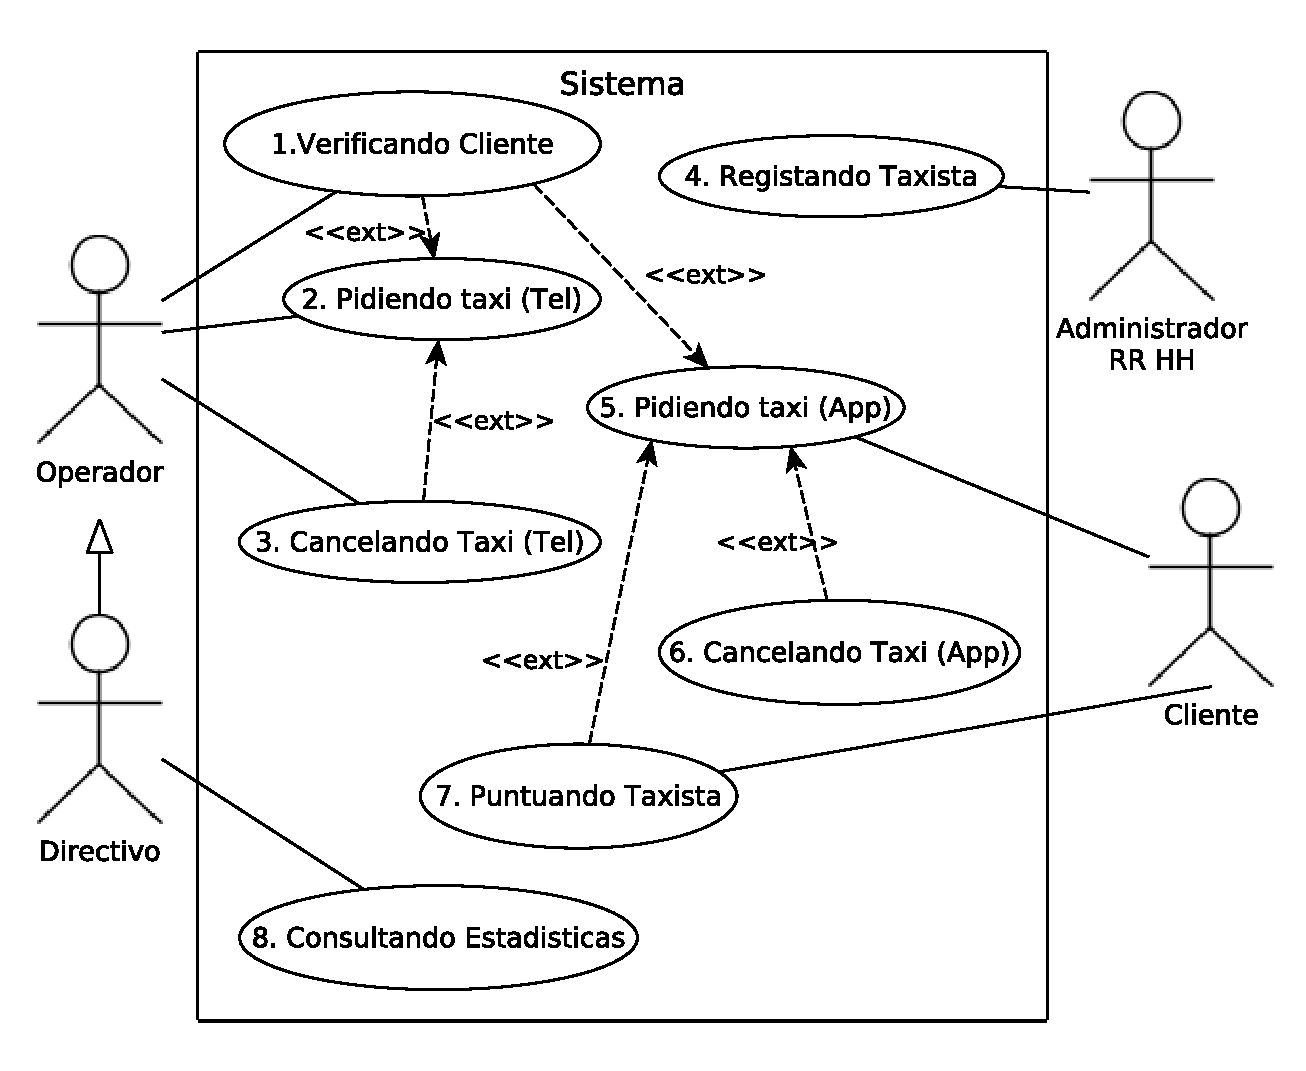
\includegraphics[scale=0.75]{diag_CasosDeUso.pdf}

En los lugares donde hubiere un O-ref en el diagrama de objetivos, decidimos tomar la alternativa m\'as fiel al enunciado original: optamos por no utilizar una remiser\'ia para los viajes regulares, y por no implementar la alternativa de los mensajes de texto.
\section{Casos de Uso}


\subsection{Caso de Uso \textit{Verificando Cliente}}
\begin{center}
\begin{tabular}{|p{10cm} | p{6cm}|}
\hline
\multicolumn{2}{|p{16cm}|}{\textbf{Descripci\'on:} Se verifica si el cliente est\'a registrado. Si no lo est\'a, se le pide los datos y se lo registra en el sistema.} \\
\hline
\multicolumn{2}{|l|}{\textbf{Actor:} Operador} \\
\hline
\multicolumn{2}{|l|}{\textbf{Pre:} -} \\
\hline
\multicolumn{2}{|p{14cm}|}{\textbf{Post:} Se verifica que el usuario est\'a registrado, y si no lo estaba se lo registra en el sistema.}\\
\hline
\textbf{Curso Normal}  & \textbf{Curso Alternativo} \\ \hline

1. El sistema solicita el nombre completo del usuario. & \\ \hline
2. El operador ingresa el nombre completo. & \\ \hline
3. El sistema busca los datos del usuario. Si no los encuentra, EXTIENDE CASO DE USO \textit{Registrando Cliente}. & \\ \hline
4. Fin caso de uso & \\ \hline
\end{tabular}
\end{center}
% NO ESTOY SEGURA SI ESTO ES CASO ALTERNATIVO O NO
% POR QUE NO ES EL CLIENTE UN ACTOR? A QUIEN LE PIDO LOS DATOS?

\subsection{Caso de Uso \textit{Pidiendo Taxi (Tel\'efono)}}
\begin{center}
\begin{tabular}{|p{8cm} | p{8cm}|}
\hline
\multicolumn{2}{|p{16cm}|}{\textbf{Descripci\'on:} } \\
\hline
\multicolumn{2}{|l|}{\textbf{Actor:} } \\
\hline
\multicolumn{2}{|l|}{\textbf{Pre:} } \\
\hline
\multicolumn{2}{|p{14cm}|}{\textbf{Post:} }\\
\hline
\textbf{Curso Normal}  & \textbf{Curso Alternativo} \\ \hline
 & \\ \hline
 & \\ \hline
 & \\ \hline
 & \\ \hline
 & \\ \hline
 & \\ \hline
 & \\ \hline
 & \\ \hline
 & \\ \hline
 & \\ \hline
\end{tabular}
\end{center}

\subsection{Caso de Uso \textit{Cancelando Taxi (Tel\'efono)}}
\begin{center}
\begin{tabular}{|p{8cm} | p{8cm}|}
\hline
\multicolumn{2}{|p{15cm}|}{\textbf{Descripci\'on:} Se cancela el pedido de un viaje pedido telef\'onicamente.} \\
\hline
\multicolumn{2}{|p{15cm}|}{\textbf{Actor:} Operador} \\
\hline
\multicolumn{2}{|p{15cm}|}{\textbf{Pre:} El viaje que se desea cancelar ya fue pedido pero todav\'ia no fue realizado. El viaje fue pedido telef\'onicamente.} \\
\hline
\multicolumn{2}{|p{14cm}|}{\textbf{Post:} El viaje es cancelado, informando al taxista de su cancelaci\'on y borr\'andolo de los viajes a realizar.}\\
\hline
\textbf{Curso Normal}  & \textbf{Curso Alternativo} \\ \hline
 & \\ \hline
 & \\ \hline
 & \\ \hline
 & \\ \hline
 & \\ \hline
 & \\ \hline
 & \\ \hline
 & \\ \hline
 & \\ \hline
 & \\ \hline
\end{tabular}
\end{center}

\subsection{Caso de Uso \textit{Registrando taxista}}
\begin{center}
\begin{tabular}{|p{10cm} | p{6cm}|}
\hline
\multicolumn{2}{|p{15cm}|}{\textbf{Descripci\'on:} Se registra a un nuevo taxista en la lista de taxistas de la empresa del sistema.} \\
\hline
\multicolumn{2}{|l|}{\textbf{Actor:} Administrador RRHH } \\
\hline
\multicolumn{2}{|p{15cm}|}{\textbf{Pre:} Se seleccion\'o un taxista para contratar, y el taxista seleccionado todav\'ia no es parte de la empresa. } \\
\hline
\multicolumn{2}{|p{15cm}|}{\textbf{Post:} Se agreg\'o al nuevo taxista a la flota de la empresa (la lista de taxistas de la empresa en el sistema). }\\
\hline
\textbf{Curso Normal}  & \textbf{Curso Alternativo} \\ \hline
1. El administrador solicita agregar a un nuevo taxista al sistema. & \\ \hline
2. El sistema pide los datos del nuevo taxista a agregar. & \\ \hline
3. El administrador ingresa los datos del nuevo taxista. & \\ \hline
4. El sistema informa que se agreg\'o correctamente al taxista a la flota. & 4.1 Si el taxista ya era parte de la flota, el sistema informa que es imposible agregarlo y retorna al paso 2. \\ \hline
5. Fin de caso de uso. & \\ \hline

\end{tabular}
\end{center}

\subsection{Caso de Uso \textit{Pidiendo Taxi (Aplicaci\'on)}}
\begin{center}
\begin{tabular}{|p{10cm} | p{6cm}|}
\hline
\multicolumn{2}{|p{15cm}|}{\textbf{Descripci\'on:} El cliente pide un taxi v\'ia la aplicaci\'on de acuerdo con sus preferencias. } \\
\hline
\multicolumn{2}{|p{15cm}|}{\textbf{Actor:} Cliente } \\
\hline
\multicolumn{2}{|p{15cm}|}{\textbf{Pre:} El cliente desea pedir un viaje y lo har\'a via la aplicaci\'on.} \\
\hline
\multicolumn{2}{|p{15cm}|}{\textbf{Post:} Un taxi se env\'ia seg\'un el pedido del cliente. Una vez que el taxi comienza a moverse, se muestra su posici\'on a trav\'es de la aplicaci\'on. }\\
\hline
\textbf{Curso Normal}  & \textbf{Curso Alternativo} \\ \hline
 & \\ \hline
 & \\ \hline
 & \\ \hline
 & \\ \hline
 & \\ \hline
 & \\ \hline
 & \\ \hline
 & \\ \hline
 & \\ \hline
 & \\ \hline
\end{tabular}
\end{center}


\subsection{Caso de Uso \textit{Cancelando Taxi (Aplicaci\'on)}}
\begin{center}
\begin{tabular}{|p{10cm} | p{6cm}|}
\hline
\multicolumn{2}{|p{16cm}|}{\textbf{Descripci\'on:} Se cancela el pedido de un viaje pedido a trav\'es de la aplicaci\'on.} \\
\hline
\multicolumn{2}{|l|}{\textbf{Actor:} Cliente} \\
\hline
\multicolumn{2}{|p{15cm}|}{\textbf{Pre:} El viaje que se desea cancelar ya fue pedido pero todav\'ia no fue realizado. El viaje fue pedido a trav\'es de la aplicaci\'on.} \\
\hline
\multicolumn{2}{|p{15cm}|}{\textbf{Post:} El viaje es cancelado, informando al taxista de su cancelaci\'on y borr\'andolo de los viajes a realizar.}\\
\hline
\textbf{Curso Normal}  & \textbf{Curso Alternativo} \\ \hline
 & \\ \hline
 & \\ \hline
 & \\ \hline
 & \\ \hline
 & \\ \hline
 & \\ \hline
 & \\ \hline
 & \\ \hline
 & \\ \hline
 & \\ \hline
\end{tabular}
\end{center}

\subsection{Caso de Uso \textit{Puntuando Taxista}}
\begin{center}
\begin{tabular}{|p{10cm} | p{6cm}|}
\hline
\multicolumn{2}{|p{16cm}|}{\textbf{Descripci\'on:} El cliente punt\'ua al taxista seg\'un su experiencia del viaje, y su opini\'on se carga en el sistema.} \\
\hline
\multicolumn{2}{|l|}{\textbf{Actor:} Cliente } \\
\hline
\multicolumn{2}{|p{15.5cm}|}{\textbf{Pre:} El cliente realiz\'o un viaje con el taxista puntuado y a\'un no lo evalu\'o por ese viaje (si realiz\'o m\'as de un viaje con el taxista, tiene que tener al menos un viaje por el que no lo puntu\'o). } \\
\hline
\multicolumn{2}{|p{14cm}|}{\textbf{Post:} La opini\'on y el puntaje del cliente sobre el taxista es cargado en el sistema. }\\
\hline
\textbf{Curso Normal}  & \textbf{Curso Alternativo} \\ \hline
1. El cliente solicita dar su opini\'on sobre un taxista. & \\ \hline
2. El sistema muestra todos los taxistas de viajes que a\'un no fueron puntuados. & \\ \hline
3. El cliente selecciona el taxista de qu\'e viaje desea puntuar. & \\ \hline
4. El sistema solicita la opini\'on y el puntaje del cliente sobre el taxista del viaje seleccionado. & \\ \hline
5. El cliente punt\'ua al taxista y opcionalmente deja un comentario escrito. & \\ \hline
6. El sistema informa que el puntaje fue cargado exitosamente. & 6.1 Si el sistema no pudo cargar el puntaje, se lo informa y se retorna al paso 2.\\ \hline
7. Fin de caso de uso. & \\ \hline

%% ESTO PERMITE QUE EVALUE MAS DE UNA VEZ AL MISMO TAXISTA

\end{tabular}
\end{center}

\subsection{Caso de Uso \textit{Consultando estad\'isticas}}
\begin{center}
\begin{tabular}{|p{10cm} | p{6cm}|}
\hline
\multicolumn{2}{|p{16cm}|}{\textbf{Descripci\'on:} Se consultan las estad\'isticas sobre la conformidad de los usuarios con el sistema y/o sobre el uso del sistema coordinando los taxis. } \\
\hline
\multicolumn{2}{|l|}{\textbf{Actor:} Directivo } \\
\hline
\multicolumn{2}{|l|}{\textbf{Pre:} - } \\
\hline
\multicolumn{2}{|p{14cm}|}{\textbf{Post:} El sistema muestra las estad\'isticas pedidas. }\\
\hline
\textbf{Curso Normal}  & \textbf{Curso Alternativo} \\ \hline
1. El directivo solicita que el sistema le muestre todas las estad\'isticas existentes. & \\ \hline
2. El sistema lista todas las estad\'isticas que puede mostrar. & \\ \hline
3. El directivo selecciona la estad\'istica que quiere conocer. & \\ \hline
4. El sistema muestra la estad\'istica solicitada y pregunta si se desea conocer otra estad\'istica. &  \\ \hline
5. El directivo informa que no desea ver m\'as estad\'isticas. & 5.1 Si desea conocer otras estad\'isticas, volver al paso 1. \\ \hline
6. Fin de caso de uso. & \\ \hline
\end{tabular}
\end{center}
%% NO ESTOY SEGURA COMO PONER LAS DOS RAMAS DEL IF

\subsection{Caso de Uso \textit{Registrando Cliente}}
\begin{center}
\begin{tabular}{|p{10cm} | p{6cm}|}
\hline
\multicolumn{2}{|p{16cm}|}{\textbf{Descripci\'on:} Se registra al nuevo cliente en el sistema.} \\
\hline
\multicolumn{2}{|l|}{\textbf{Actor:} Operador} \\
\hline
\multicolumn{2}{|l|}{\textbf{Pre:} El cliente a registrar no est\'a a\'un en el sistema.} \\
\hline
\multicolumn{2}{|p{14cm}|}{\textbf{Post:} El nuevo cliente est\'a registrado en el sistema.}\\
\hline
\textbf{Curso Normal}  & \textbf{Curso Alternativo} \\ \hline
1. El sistema solicita los datos del nuevo cliente. & \\ \hline
2. El operador ingresa todos los datos personales del cliente. & \\ \hline
3. El sistema informa que el nuevo cliente fue registrado en el sistema. & 3.1 Si el sistema no pudo agregar al nuevo cliente, se informa este hecho y se va al paso 1. \\ \hline
4. Fin caso de uso & \\ \hline
\end{tabular}
\end{center}

\section{Diagrama de Clases}

\section{OCL}

\section{FSM}

La primer m\'aquina de estado refleja los estados posibles de la terminal en taxi. El taxi
puede estar: inactivo (no puede recibir viajes), activo (donde puede aceptar viajes de la calle o le pueden llegar pedidos), 
u ocupado si es que est\'a realizando un viaje. El otro posible estado es cuando acepta o rechaza los pedidos de taxi que le envian.

La segunda FSM refleja los cambios del sistema cuando se asignan los viajes, se aceptan, se rechazan y las actualizaciones de ubicaci\'on de cada
taxi. Tambi\'en muestra cuando esta disponible, no disponible o inactivo un taxi determinado.

\begin{center}
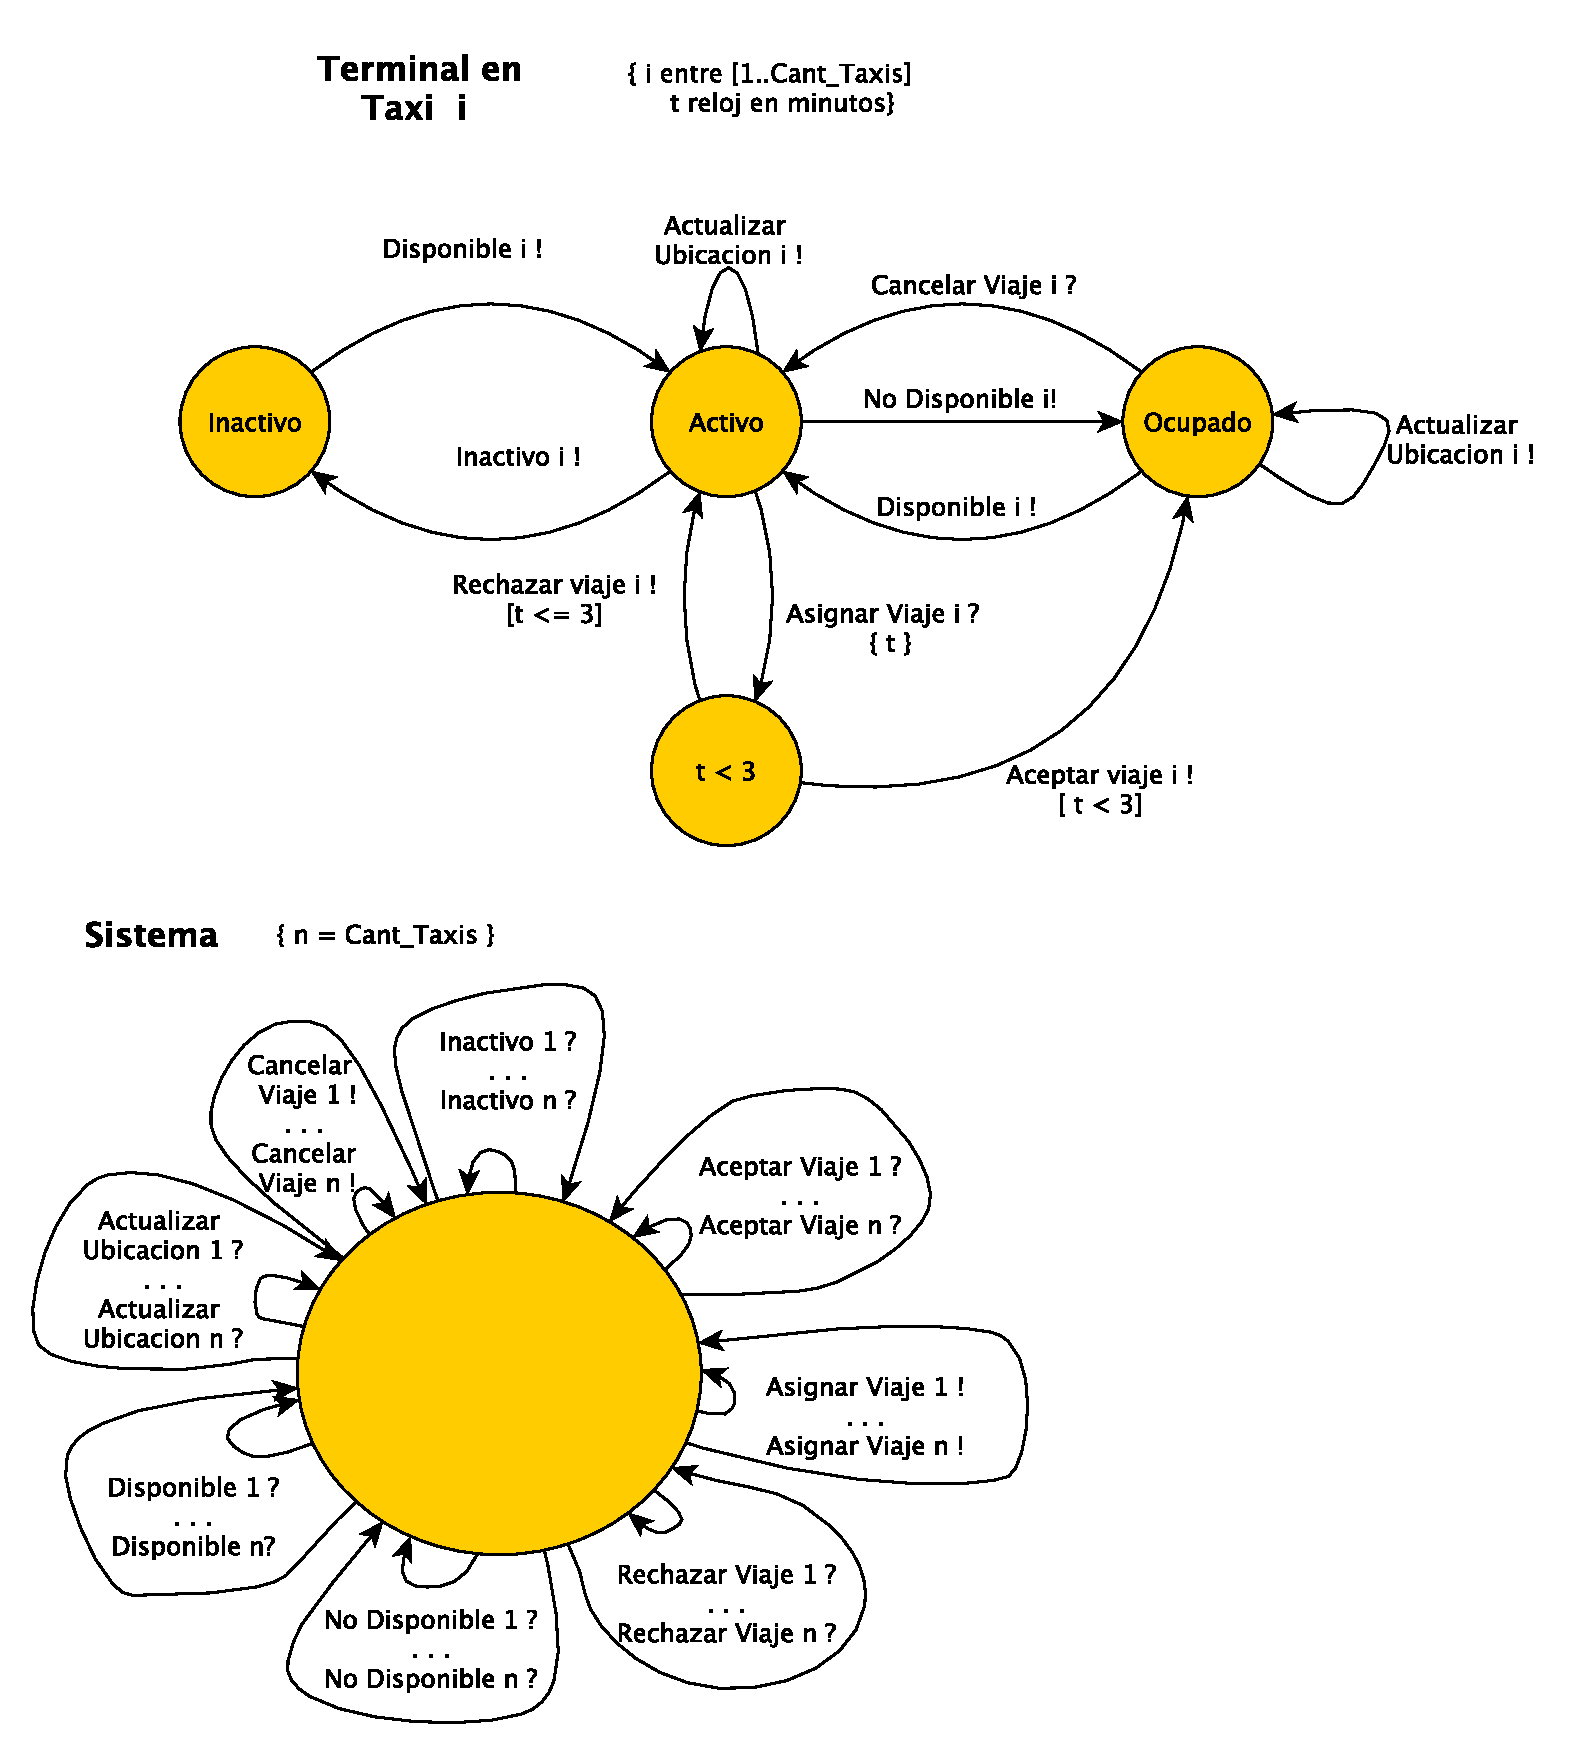
\includegraphics[scale=0.6]{diag_FSM.pdf}
\end{center}


\section{Diagramas de Actividad}

\end{document}
